% standard
\documentclass[a4paper,11pt]{article}
\usepackage[utf8]{inputenc}
\usepackage[ngerman]{babel}

\usepackage{titlesec}
\usepackage{tocbibind}
\renewcommand{\listoffigures}{\begingroup
\tocsection
\tocfile{\listfigurename}{lof}
\endgroup}

\setcounter{secnumdepth}{5}
\setcounter{tocdepth}{5}
\titleformat{\paragraph} {\normalfont\normalsize\bfseries}{\theparagraph}{1em}{}
\titlespacing*{\paragraph}
{0pt}{3.25ex plus 1ex minus .2ex}{1.5ex plus .2ex}

%for linkt page numbers in table of content
\usepackage[linktocpage=true]{hyperref}

\usepackage{enumitem}

\hypersetup{%
unicode,pdffitwindow,
pdfkeywords = {pdf, LaTeX, hyperref, thumbnails},
pdfauthor = {Brüder Grimm},
bookmarksopen = true,
bookmarksnumbered = true,
pdfcenterwindow=true,
pdffitwindow = true,
pdfstartview=FitBV,
pdfcreator = {pdflatex},
colorlinks=true, breaklinks=true, %
urlcolor=magenta, % color for \url
filecolor=cyan, % color for file
linkcolor=black, % color for \ref
citecolor=magenta, %color for \cite
menucolor=darkblue,
breaklinks=true,anchorcolor=green
}

% geometry
\usepackage{geometry}
\geometry{ headsep=20pt,
headheight=20pt,
left=21mm,
top=15mm,
right=21mm,
bottom=15mm,
footskip=20pt,
includeheadfoot}

% for using wrapfigures
\usepackage{wrapfig}

% header and footer
\usepackage{datetime}
\newdateformat{dmy}{%
\THEDAY.~\monthname[\THEMONTH] \THEYEAR}
\usepackage{fancyhdr}
\pagestyle{fancy}
\lhead{Noah Vogt}
\chead{}
%\rhead{\dmy\today}
\lfoot{}
\cfoot{Gymnasium Kirschgarten, Basel (CH)}
\rfoot{Seite \thepage}
\renewcommand{\footrulewidth}{.4pt}

% fix figure positioning
\usepackage{float}

% larger inner table margin
\renewcommand{\arraystretch}{1.4}

% no paragraph indent
\setlength{\parindent}{0em}

%for spacing
\usepackage{setspace}
%\renewcommand{\baselinestretch}{1.5}
%\onehalfspacing

% graphics package
\usepackage{graphicx}

% use sans serif font
\usepackage{tgheros}
\usepackage{mathptmx}

\usepackage[font={small,it}]{caption}

% for quotes
\newenvironment{nicequote}[2]{
    \begin{center}\begin{quote}\textit{#1}\\\par\raggedleft--- {#2}
    }{
    \end{quote}\end{center}
}


% using \say{} for easier quoting
\usepackage{dirtytalk}

% for code snippits
\usepackage{listings}
\usepackage{color}
\usepackage{xcolor}

\definecolor{dkgreen}{rgb}{0,0.6,0}
\definecolor{gray}{rgb}{0.5,0.5,0.5}
\definecolor{mauve}{rgb}{0.58,0,0.82}
\definecolor{background}{rgb}{0.36,0.36,0.36}
\definecolor{shpurple}{HTML}{C301FF}
\definecolor{shgreen}{HTML}{3CFF00}

\lstset{
    numbersep=3pt,
    keywordstyle=\color{blue},
    commentstyle=\color{dkgreen},
    stringstyle=\color{mauve},
    breaklines=true,
    numbers=left,
    numberstyle=\scriptsize\color{black},
    frame=none,
    basicstyle = \small\ttfamily,
    breaklines=true
    breakatwhitespace=false,
    columns=flexible,
    xleftmargin=0.5cm,framesep=8pt,framerule=0pt,
    aboveskip=3mm,
    morekeywords={*, factorial, sum, erlang},
    keywordstyle=\color{shpurple}\textbf,
    commentstyle=\color{shgreen}\textit,
    stringstyle=\color{shred}   belowskip=3mm,
}

%\usepackage[backend=biber,style=apa]{biblatex}
\usepackage[
backend=biber,
style=alphabetic,
sorting=ynt,
]{biblatex}
\addbibresource{lit/refs.bib}

\usepackage{csquotes}

\begin{document}


\begin{titlepage}

	\centering

    \vspace{5cm}
    \vspace{0.1cm}
	{\huge\bfseries Portfolioarbeit Ergänzungsfach Informatik \par}
	\vspace{0.5cm}
	{\Large eine Arbeit von \par}
	{\Large Noah J. Vogt \par}
    {\Large aus der Klasse 4cg \par}
    \vspace{0.5cm}

    %\begin{figure}[H]
    %    \centering
    %    %\includegraphics[width=.8\textwidth]{../logo/version3d.png}
    %    \includegraphics[width=.7\textwidth]{../logo/version3d.png}
    %\end{figure}

    \vspace{0.5cm}
    {\Large Fachlehrperson: Victor Yakhontov \par }
    \vspace{0.5cm}
	{\large Geschrieben im Jahr 2022 \par}
    {\large Gymnasium Kirschgarten, Basel-Stadt CH \par}

\end{titlepage}

\tableofcontents
\pagebreak

\section{Einleitung}
\subsection{Darstellung}
Das Produkt dieser Portfolioarbeit ist ein ausführbares Programm mit geografischer Oberfläche, welches ein volles Jass-Kartendeck - also 52 Karten - darstellt und eine Mischfunktion anbietet.\\

\begin{figure}[H]
    \centering
    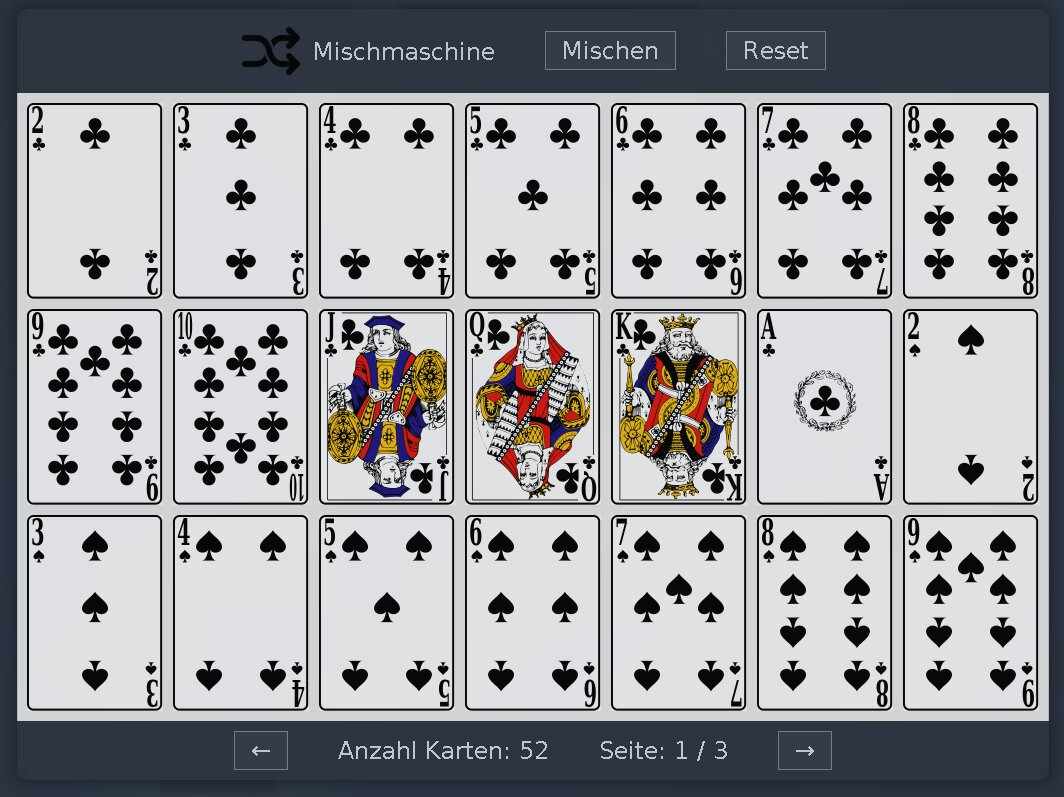
\includegraphics[width=.7\textwidth]{media/early-screenshot.jpg}
    \caption{Spielkarten}
\end{figure}

Zuerst sind die Karten in sortierter Reihenfolge dargestellt, sie werden erst durch das Drücken auf den \say{Misch}-Button gemischt. Dieser Vorgang lässt sich beliebig oft wiederholen durch erneutes Drücken des Knopfes durch den Nutzer. Um wieder zum sortierten Anfangszustand zurück zu gelangen, kann man den \say{Reset}-Button drücken.\\

Da man die Karten alle relativ klein darstellen müsste, um das ganze Kartendeck gleichzeitig zeigen zu können, wurde sich entschieden, die Kartenanzeige in verschiedene Fenster einzuteilen. So gibt es drei Seiten, mit der man durch anklicken der Arrowbuttons navigieren kann. Jede Seite besteht aus einem Rasterlayout bestehend aus drei Reihen und sieben Spalten. Die Karten werden von oben links nach unten rechts gefüllt, doch dazu später mehr.\\


\subsection{Abgrenzung}
Es gibt einige Einschränkungen, welche den Rahmen dieser Arbeit setzen:

\begin{itemize}
    \item \textbf{Die Grundbedingungen} Es sollen Abgabetermine und formale Vorgaben erfüllt werden, wie definiert im Arbeitsauftrag.
    \item \textbf{Die Aufgabestellung} Diese gilt zu beachten und soll erfüllt werden mit all ihren Teilaufgaben. Viel weiter darüber hinaus soll die App funktionstechnisch also nicht gehen, stattdessen soll vor dem Hinzufügen neuer Features sorgfältig abgewogen werden, ob diese zu weit gehen oder noch im Sinne der Aufgabenstellung zu verstehen sind und somit im Rahmen sind.
    \item \textbf{Die Programmiersprache} Zur Lösung der Aufgabestellung und Programmierung der App soll die altbekannte Sprache \texttt{Java} verwendet werden. Davon ausgenommen ist hier aber das Buildscript (\texttt{build.sh}), welches das Programm kompiliert und eine \texttt{.jar}-Executable ausgibt.
\end{itemize}

\subsection{Vorausschau}

Im darauffolgenden Hauptteil dieser Portfolioarbeit wird zuerst genauer auf die Aufgabestellung eingegangen, analysiert und interpretiert. Dies ist ein wichtiger Schritt, denn er soll den weiteren Ablauf des Projekts bestimmen.\\

Als nächstes wird der grobe Lösungsansatz vorgestellt, und immer weiter vertieft. Dazu wird sich unter anderem bedient an Codebeispielen, Programmablaufdiagrammen und Screenshots, um durch die grafische Darstellung die Konzepte besser anschaulich zu machen.\\

Ebenso wird auch auf die Wahl von Bibliotheken und relevanten Programmierwerkzeugen eingegangen. Diese werden je nach dem kurz vorgestellt, mit Alternativen verglichen und der Entscheid begründet.\\

Abschliessend erfolgt der Rückblick auf das Projekt und der Autor bewertet die Erfahrungen, das Gelernte und die Resultate.


\section{Hauptteil}

\subsection{Aufgabestellung und Interpretation}

\textit{\textbf{1a)} Implementieren Sie zunächst eine ausführbare (d.h. mit einer main()–Methode) Klasse Karten, welche die Karten des Kartenspiels erzeugen und grafisch (s. Abb. 1) auslegen kann.}

\begin{figure}[H]
    \centering
    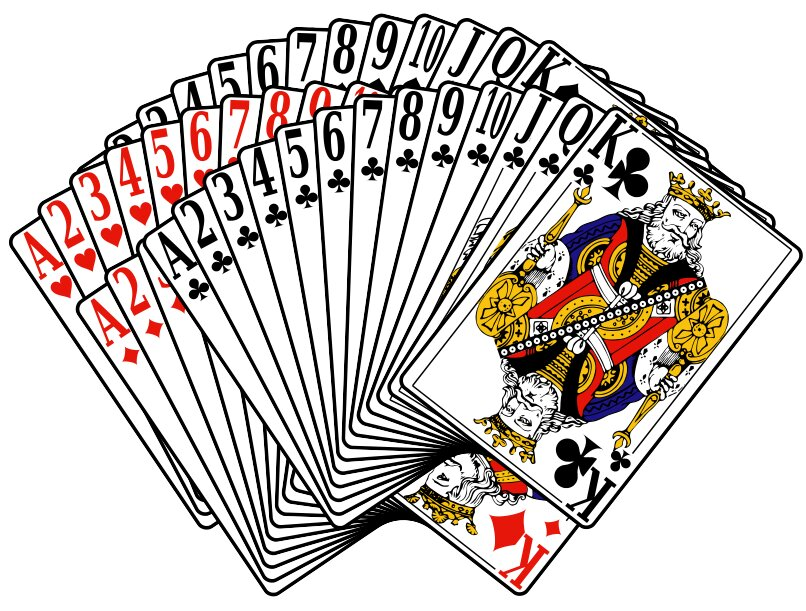
\includegraphics[width=.45\textwidth]{media/spielkarten.jpg}
    \caption{Spielkarten}
\end{figure}

Hier im Beispielbild (Abb. 1) wurde die Auslegung der Karten übereinanderliegend dargestellt, doch es wurde sich für eine nicht überlappende Darstellung der Karten entschieden, das die besser zu einem grafischen Programm passe aufgrund erhöhter Lesbarkeit und wesentlich geringerem Arbeitsaufwand.\\

Es ist nicht klar gegeben, ob die ausführbare Klasse \texttt{Karten} mit \texttt{main()}-Methode als einzelnes Source File dastehen soll oder ob darin verwendete Module auch in anderen Source Files gespeichert werden können. Es wurde sich für diese Arbeit entschieden, das letztere zu wählen, um einen besser strukturierten Gesamtquellcode zu erreichen.\\

\textit{\textbf{1b)} Für das Kartenspiel benötigen Sie auch eine Mischmaschine, welche die Karten mischen kann. Objekte der entsprechenden Klasse MischMaschine müssen in der Lage sein:
\begin{enumerate}[label=\roman*.]
    \item Karten aufzunehmen,
    \item die enthaltenen Karten zu mischen,
    \item alle enthaltenen Karten zu durchlaufen.
\end{enumerate}
Sie lernen die Klasse \texttt{java.util.ArrayList} kennen und stellen dadurch fest, dass diese bereits die
Anforderungen (i) und (iii) über die beiden Methoden \texttt{add()} und \texttt{Iterator()} erfüllt. Für die Realisierung der Klasse \texttt{MischMaschine} können Sie also grundsätzlich die Klasse \texttt{ArrayList} und das Konzept der Vererbung nutzen. Um die Anforderung (ii) zu implementieren, müssen Sie zusätzlich Ihre eigene Methode \texttt{mischen()} schreiben (s. die Methode \texttt{java.util.Collections.shuffle()} aus der Klasse \texttt{java.util.*}), die das Mischen tatsächlich realisiert, und zu Ihrer Klasse hinzufügen.
Implementieren Sie auf dieser Weise die externe Klasse MischMaschine, die Objekte der Hauptklasse \texttt{Karten} aufnehmen, mischen und durchlaufen kann.}\\

Dass Objekte der Klasse \texttt{MischMaschine} in der Lage sein sollen (i) - (iii) zu erfüllen ist verständlich, doch da jedoch die Klasse eine grafische Oberfläche starten soll, wird es als sinnvoller empfunden diese drei Punkte durch die Unterklasse resp. Datentyp-Klasse \texttt{KartenDeck} welche wiederum Daten der Datentyp-Klasse \texttt{Karte} bearbeitet. Dies steht ja nicht im Widerspruch zur Aufgabenstellung, sondern eine Interpretation.\\

\textit{\textbf{1c)}: Ändern Sie die Hauptklasse Karten so ab, dass sie alle erzeugten Karten des Kartenspiels an die Klasse MischMaschine übergibt. Die MischMaschine soll die Karten mischen und
anschliessend sie an die Hauptklasse Karten in der gemischten Reihenfolge zurückgeben, wo sie schlussendlich auf den Bildschirm im grafischen Interface ausgelegt werden.}\\

Hier macht es relativ wenig Sinn nach Ansicht des Autors dieser Arbeit, die Hauptklasse \texttt{Karten} direkt zu bearbeiten, um die im grafischen Interface abgebildeten Karten zu mischen. Denn solch eine Änderung sollte in der jeweiligen aus der Klasse \texttt{Karten} gecallten Klasse geschehen, im Falle der hier präsentierten Lösung ist das in der Klasse \texttt{MainWindow}.\\

Auch dass die zur Mischung stehenden Karten an die Klasse \texttt{MischMaschine} abgegeben werden soll, erscheint auch nicht direkt sinnvoll. In dieser Lösung wird das Kartendeck im User Interface in einer Instanz der Klasse \texttt{KartenDeck} gespeichert und die Mischfunktion als Methode dieser Klasseninstanz einfach gecallt.



\subsubsection{Bewertung}
Vom Autor dieser Arbeit wird diese Aufgabe als doch recht sinnvoll angesehen. Einerseits ist das Handling eines Kartenspiels resp. eines Kartendecks ein recht passender Fall, wo man die Prinzipien der OOP-Konzepts (Objekt-Orientierten Programmierung) anwenden kann: So erschien es sinnvoll eine Klasse \texttt{Karte} zu schreiben um den Datentyp einer Karte als Objekt darzustellen inklusive Getter- und Settermethoden und passenden Attributen. Ein Kartendeck wäre dann eine Klasse welche eine \texttt{ArrayList} ist, welche Objekte der Klasse \texttt{Karte} aufnehmen, und passende Methoden zu deren Manipulation bieten (Karten hinzufügen, entfernen, mischen, etc.). Ein paar OOP-Konzepte wurden im Laufe des Unterrichts im Ergänzungsfach Informatik schon angeschnitten, weshalb es nach der Meinung des Autors auch schön ist, diese wiederverwenden zu können. \\

Was auch im Unterricht behandelt wurde, sind simple grafische Interfaces mit der Flanagan-Bibliothek und der der \texttt{javax.swing}-Bibliothek. Nach der Erinnerung des Autors geschah dies in der Form von In- und Output Popup-Fenstern und Filepickern. Diese und die Swing-Bibliothek konnten auch wieder verwendet werden für die Erstellung der grafischen Oberfläche des Programmes.\\

Auf die Schlussfolgerungen und Reflexionen auf die Arbeit als gesamtes wird noch später im letzten Punkt genauer eingegangen, doch die Arbeit erschien dem Autor ausgewogen bezüglich Machbarkeit, Aufwand, Themenbereichen (Karten Backend und GUI Frontend). Ein Kritikpunkt ist aber, dass die Namen der Klassen - \texttt{Karten} und \texttt{MischMaschine} - vorgegeben waren, denn da es nach Ansicht des Autors dieses Portfolios seine kreativen Freiraum bezüglich Quellcode-Struktur und Klassenbenennung. Gegeben, bei dieser Aussage befindet man sich auf hohem Niveau der Kritik.

\subsection{Lösungsansatz}

\subsubsection{Grobe Übersicht}
\begin{figure}[H]
    \centering
    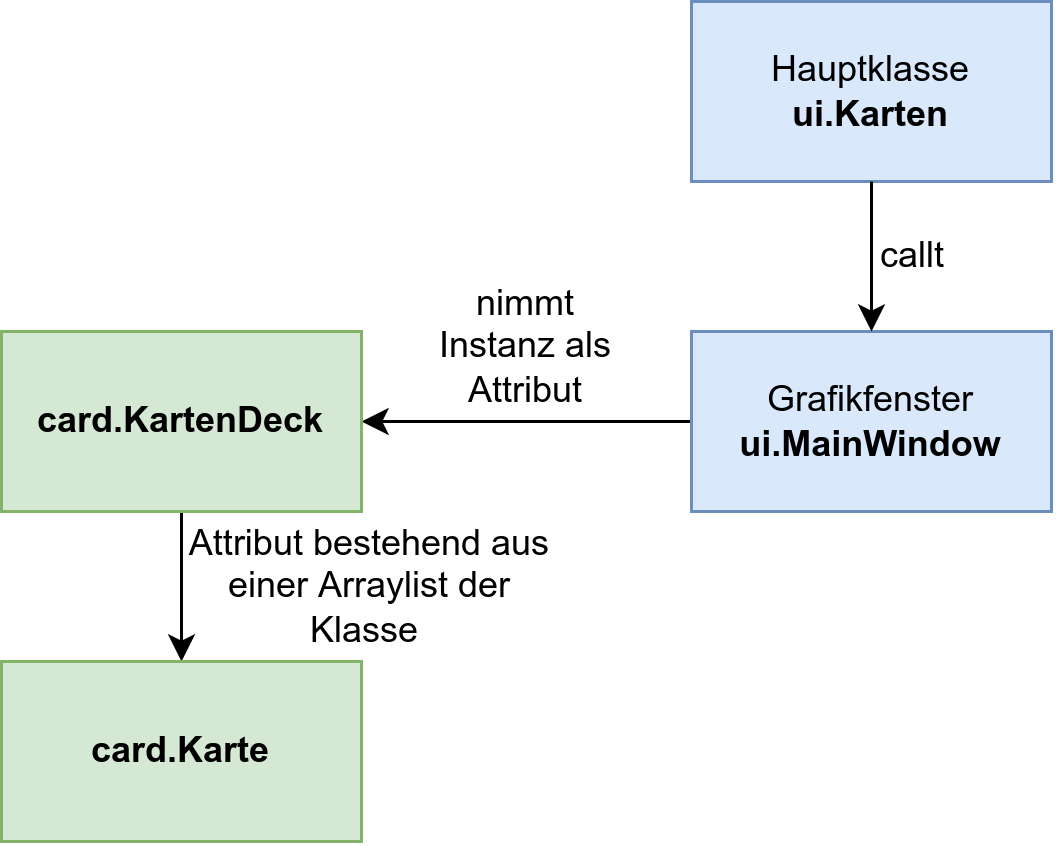
\includegraphics[width=.6\textwidth]{media/grober-ansatz.png}
    \caption{Spielkarten}
    % TODO: mention 3 panels
\end{figure}

Wie in der obigen Abbildung ersichtlich, wird in der Hauptklasse \texttt{Karten} durch das \texttt{SwingUtilities.invokeLater()}-Environment ausgeführt, welches den einzigen Nutzen hat, das Grafikfenster zu starten, welches in der Klasse \texttt{MainWindow} geschrieben ist.\\

Das Grafikfenster besteht aus verschiedenen Komponenten der AWT- und Swing-Library, doch darauf wird später im Text noch genauer eingegangen. Grob ist das Programm aber eingeteilt in ein Top-Panel, Bottom-Panel und eine Kartenansicht dazwischen.\\

Um mit dem Kartendeck im Grafikfenster sinnvoll umgehen zu können, wurde ein Objekt resp. eine Klasse names \texttt{KartenDeck} erstellt, welche alle nötigen Methoden besitzt für die Manipulation des Attributs, einer \texttt{ArrayList} des Typs \texttt{Karte}.

\subsubsection{Grafisches Interface}
% TODO: insert irl plan

Um ein Kartenspiel grafisch darzustellen wurde überlegt, es muss ein Fenster her, das in der Lage ist alle 52 Karten des Decks darzustellen. Und das wie schon bei der Aufgabeninterpretation erwähnt, am besten ohne Überlappungen von Karten.

JComponents

\subsubsection{Datenklasse \texttt{Karte}}
Um eine Sache in ein Datenobjekt zu übersetzen, muss man sich erst einmal überlegen, was für Eigenschaften eine Spielkarte so besitzt. Da wären zuerst die \textit{Kartenwerte} von 2 bis Ass und die sogenannten \textit{Kartenfarben} Pik, Karo, Herz und Kreuz. Mit diesen beiden Eigenschaften kann eine Karte \textit{eindeutig} definiert werden. Diese beiden Karteneigenschaften sollen dann dementsprechend Attribute der Klasse \texttt{Karte} sein.\\

Da die Kartenfarbe nur vier feste, gleichwertige Werte annehmen kann, welche sich am besten durch ihren Namen referenzieren lassen, scheint hier die Nutzung eines \texttt{enum}s angebracht. Im Code sieht dass dann so aus:\\ % TODO: insert enum / Karte.java attributes lstlisting

\lstset{language=java}
\begin{lstlisting}
    public enum Farbe {
        KREUZ, PIK, KARO, HERZ;
    }
\end{lstlisting}


Die Kartenwerte bestehen ja aus \say{2}, \say{3}, \say{4}, \say{5}, \say{6}, \say{7}, \say{8}, \say{9}, \say{10}, \say{Bauer}, \say{Dame}, \say{König}, \say{Ass}. Diese sind im Gegensatz zu den Karten nicht gleichwertig und lassen sich ganzzahligen Werten zuordnen. Für dieses Projekt sind diese wie folgt definiert:

\begin{table}[H]
\centering
\begin{tabular}{|c|c|}
    \hline
    \textbf{Kartenwert} & \textbf{Integer Wert}\\
    \hline
    \say{1} & \texttt{1}\\
    \hline
    \say{2} & \texttt{2}\\
    \hline
    \say{3} & \texttt{3}\\
    \hline
    \say{4} & \texttt{4}\\
    \hline
    \say{5} & \texttt{5}\\
    \hline
    \say{6} & \texttt{6}\\
    \hline
    \say{7} & \texttt{7}\\
    \hline
    \say{8} & \texttt{8}\\
    \hline
    \say{9} & \texttt{9}\\
    \hline
    \say{10} & \texttt{10}\\
    \hline
    \say{Bauer} & \texttt{11}\\
    \hline
    \say{Dame} & \texttt{12}\\
    \hline
    \say{König} & \texttt{13}\\
    \hline
    \say{Ass} & \texttt{14}\\
    \hline
\end{tabular}
\end{table}


\subsubsection{Datenklasse \texttt{KartenDeck}}

\subsection{Vorstellung und Erklärung}
\subsubsection{Top Panel}
\begin{figure}[H]
    \centering
    
\includegraphics[width=.9\textwidth]{media/top-panel.jpg}
    \caption{Screenshot: Bottom Panel}
\end{figure}

\subsubsection{Bottom Panel}
\begin{figure}[H]
    \centering
    
\includegraphics[width=.9\textwidth]{media/bottom-panel.jpg}
    \caption{Screenshot: Bottom Panel}
\end{figure}

\subsubsection{Card Panel}
\begin{figure}[H]
    \centering
    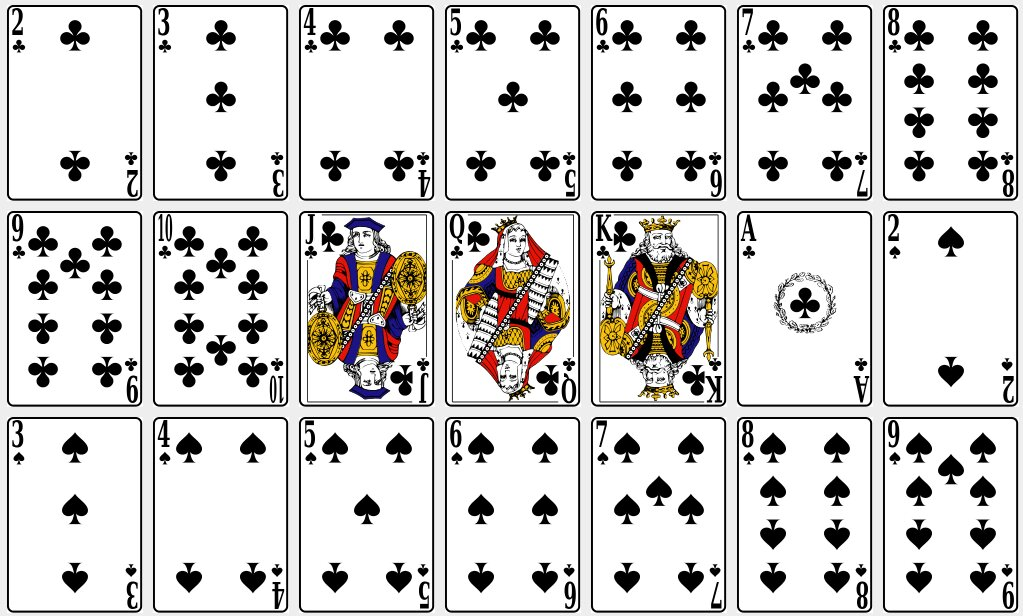
\includegraphics[width=.9\textwidth]{media/card-panel.jpg}
    \caption{Screenshot: Card Panel}
\end{figure}

\subsection{Verwendete Tools}

\subsection{Abschluss / Rückblick}

\end{document}
